\clearpage
\section{Autonomous Vehicles and Robots}

Autonomous robots or vehicles can work for an extended period of time gathering information from its surroundings to be able to work without human intervention. The robot or vehicles gathers different kinds of data, depending on what the goal of the robot it.Positional data can be utilized for navigation and path finding in a known and unknown environment. Intelligent autonomous devices are able to adapt to changes happening in its surroundings.
Currently there are many robots on the market that are self-reliant, ranging from autonomous vacuum cleaner to drones and helicopters. \cite{autonomousbasic}

Simple autonomous robots use ultrasonic sensors or infrared to manipulate itself if it detects obstacles. The is useful for obstacle avoidance and mapping of unknown areas, where the robot through a reference point can pin-point the obstacles it has encountered along the way.
More advanced robots use vision to grant them the ability to see their surroundings, algorithms analyse the camera data and gives the robot depth perception, which grants the robot the ability to instantly identify objects and locate them immediately.\cite{obstacles}

There exists two kinds of autonomous robots, a single computer autonomous robot and insect robots. The single computer autonomous robot uses its own on-board computing unit to do its computations and decisions, whereas the the insect robots are a fleet a many robots who are controlled by a single separate computing unit.
The advantage of having a single computer autonomous robot is that the tasks it performs can be done using more computer resources. It has the possibility of utilizing the computing power to its full potential, instead of relying on a separate unit that is also making decisions and calculations for many other robots.
The individual robot in the insect family is simple, but the whole robot fleet can be advanced and possibly perform sophisticated tasks, that a require multiple simpler robots.\cite{singleandinsect}


\clearpage
\section{Path finding and mapping}

Pathfinding is done by a computer, where it uses plotting to find the shortest path between two different points. It can be viewed as a more efficient way of navigating a maze.
There exists pathfinding algorithms that are used for software simulations, but also for mobile robot navigation. 

A common pathfinding algorithm is A* (A star) and its extended version D*.
%Needs some more transitioning information

\begin{figure}[H]
\centering
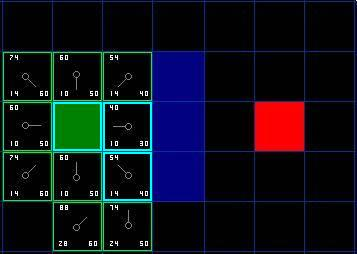
\includegraphics[width=.7\linewidth]{images/aStar2.jpg}
\caption{Upper-left number is F, Lower-left G and Lower-right H}
\label{fig:sub2}
\end{figure}

The A* algorithm is most commonly used in video games. The algorithm determines that cost of movement from the start to the given generated destination(G), in relation to the estimated cost of movement to its final destination(H). Based on the current destination the possible surrounding paths are analysed and the path with the F value(F = G + H)becomes the chosen path.\cite{astar}



%maybe add one of the block images from (good source on A*) http://www.policyalmanac.org/games/aStarTutorial.htm
%Intro to A* http://www.raywenderlich.com/4946/introduction-to-a-pathfinding
%Possible more A* information http://heyes-jones.com/astar.php
%Robots using A*? http://www.pdx.edu/computer-science/sites/www.pdx.edu.computer-science/files/TR%2012-02.pdf
%Robots using A* for navigation? http://ais.informatik.uni-freiburg.de/publications/papers/thesis_bennewitz.pdf


%D*, the extended version of A*
%Information regarding D*
%http://www.frc.ri.cmu.edu/~axs/dynamic_plan.html
%http://www.frc.ri.cmu.edu/~axs/doc/icra94.pdf
%http://idm-lab.org/project-a.html


Simple autonomous robots navigate by the use of infrared LEDs or by the use of photo-resistors and LEDS, by following lines drawn on a surface.\\
%http://www.ikalogic.com/line-tracking-sensors-and-algorithms/ <-- for the line tracking 
Some autonomous robots and vehicles use multiples of different range sensors and other sensory equipment, to map and locate themselves in indoor and outdoor environments. The map that is generated can be used to keep track of static items in the environment such as structures and difference in terrain, but the map also distinguishes non-static items such as humans and other moving objects. Since the maps are created by the vehicle itself whilst exploring, this technology can be used with or without GPS\cite{rangesens}\cite{rangesensarc}. 

\begin{figure}[H]
	\centering
	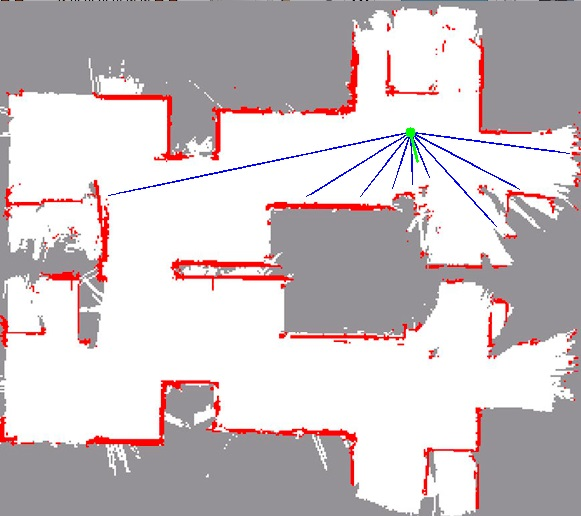
\includegraphics[scale=.7]{images/laserrangemap.jpg}
	\caption{Laser range map}
	\label{fig:laserrangemap}
\end{figure}
%http://www.jaychakravarty.com/?p=75

Laser range finders and sonar arrays are used to navigate and determine the shortest possible path to a given destination. The sensor equipment is used to give the autonomous robot a sense of distance towards objects in an environment, giving it vital data regarding optimal travel directions.\cite{lasersonar}


%http://www.kuka-labs.com/en/service_robotics/mobile_robotics/autonomous_navigation/

%Advanced imagery stufferino
%http://ilab.usc.edu/publications/doc/Siagian_etal13icra.pdf

%Misc
%http://www.doc.ic.ac.uk/~nd/surprise_97/journal/vol4/jmd/
%http://www.doc.ic.ac.uk/~nd/surprise_97/journal/vol1/jmd/


